\documentclass{beamer}
\usepackage{microtype}
\usepackage{default}

\usetheme{simple}
\usepackage{fontspec}
\usepackage{graphicx}
\usepackage[utf8]{inputenc}
\usepackage[justification=centering]{caption}
\usepackage{subcaption}
\usepackage{listings}
\setmainfont{Fira Sans}
\setsansfont{Fira Sans}
\setmonofont{Fira Mono}
\captionsetup[subfigure]{labelformat=empty}
\captionsetup[figure]{labelformat=empty}
\setbeamertemplate{caption}{\raggedright\insertcaption\par}
\setbeamerfont{frametitle}{size=\LARGE}
\newfontfamily\DejaSans{DejaVu Sans}
\setbeamerfont{title}{family=\texttt,size=\huge}
\usepackage[scale=2]{ccicons}
\title{The i-score interactive sequencer}
\subtitle{an intermedia sequencer for interactive scenarios authoring}
\date{\today}
\author{Jean-Michaël Celerier, Théo de la Hogue}
\institute{LaBRI, Blue Yeti, GMEA }
\date{January 30, 2016}

\newsavebox{\codebox}% For storing listings
\begin{document}
    
\maketitle

\begin{frame}
    \frametitle{The problem}    
    \Large
    \begin{itemize}
    	\item A lot of tools for entirely fixed, "rendered" content.
    	\item A lot of tools for entirely interactive content (artistic installations).
    	\item What goes in between ?    	
    \end{itemize}    
\end{frame}

\begin{frame}
    \frametitle{Example installations}        

    \begin{figure}
        \centering
        \includegraphics[width=0.9\textwidth]{images/futuroscope.jpg}
        \caption{Futuroscope, France. Blue Yeti}
    \end{figure}
\end{frame}


\begin{frame}
    \frametitle{Example installations}       
    
    \begin{figure}
    	\centering
    	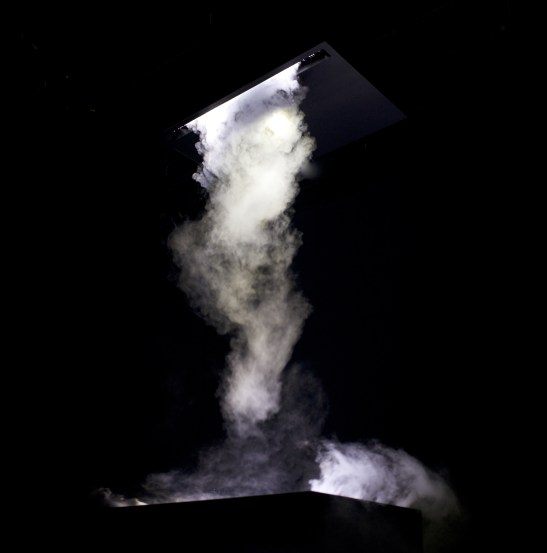
\includegraphics[width=0.6\textwidth]{images/tumbleweed.jpg}
    	\caption{Tumbleweed, Les Baltazars}
    \end{figure}
\end{frame}

\begin{frame}
    \frametitle{Screenshot}    
    \begin{figure}
    	\centering
    	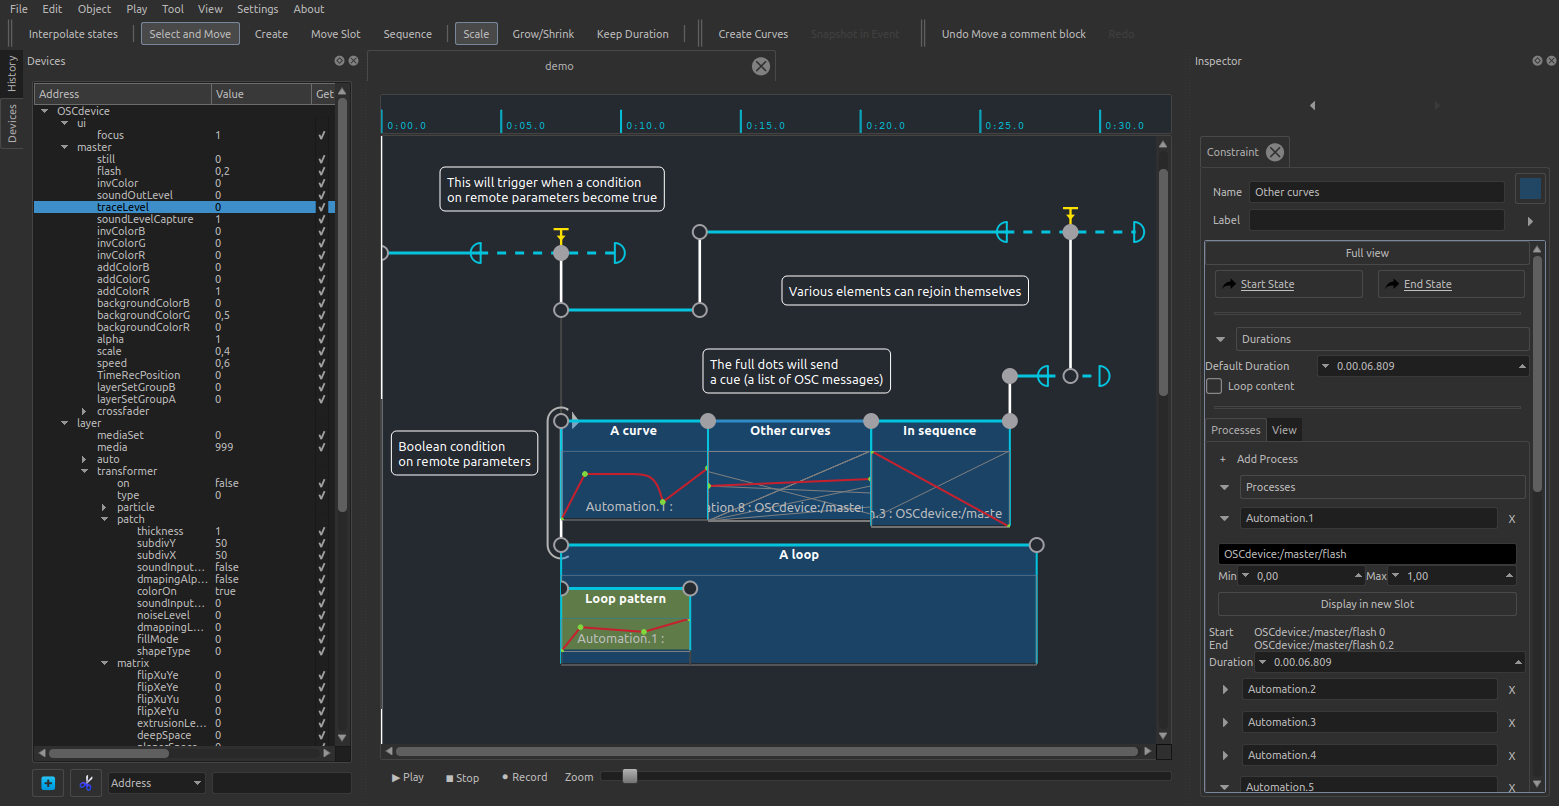
\includegraphics[width=\textwidth]{images/iscore.png}
    	\caption{i-score}
    \end{figure}    
\end{frame}


\begin{frame}
    \frametitle{Contributors, Companies, Agencies involved}
    \begin{figure}[htbp]
    \begin{subfigure}[b]{0.30\textwidth} 
        \centering
        
\begin{tikzpicture}[scale=.05]

\pgfmathsetmacro\bleulabriR{0/255}
\pgfmathsetmacro\bleulabriG{114/255}
\pgfmathsetmacro\bleulabriB{185/255}

\pgfmathsetmacro\vertlabriR{10/255}
\pgfmathsetmacro\vertlabriG{177/255}
\pgfmathsetmacro\vertlabriB{134/255}

\pgfmathsetmacro\rougelabritopR{162/255}
\pgfmathsetmacro\rougelabritopG{47/255}
\pgfmathsetmacro\rougelabritopB{50/255}

\pgfmathsetmacro\rougelabrimiddleR{178/255}
\pgfmathsetmacro\rougelabrimiddleG{117/255}
\pgfmathsetmacro\rougelabrimiddleB{99/255}

\pgfmathsetmacro\rougelabribottomR{230/255}
\pgfmathsetmacro\rougelabribottomG{206/255}
\pgfmathsetmacro\rougelabribottomB{196/255}


\definecolor{bleulabri}{rgb}{\bleulabriR, \bleulabriG, \bleulabriB}
\definecolor{vertlabri}{rgb}{\vertlabriR, \vertlabriG, \vertlabriB}
\definecolor{rougetoplabri}{rgb}{\rougelabritopR, \rougelabritopG,
 \rougelabritopB}
\definecolor{rougemiddlelabri}{rgb}{\rougelabrimiddleR,
 \rougelabrimiddleG, \rougelabrimiddleB}
\definecolor{rougebottomlabri}{rgb}{\rougelabribottomR,
 \rougelabribottomG, \rougelabribottomB}

\def\rectanglepath{-- ++(0cm,38.5cm)-- ++(10cm,0cm)--
 ++(0cm,-30.3cm)-- ++(13cm,0cm)-- ++(-2cm,-8.2cm)-- cycle}


\shade[top color=rougetoplabri!95!black,bottom
 color=rougebottomlabri!15!white!95!black,middle
 color=rougemiddlelabri!90!white!98!black,shading=axis,
shading angle=-135] (19.25, 19.25) circle (6.75cm);

\fill[fill=bleulabri] (0,0) \rectanglepath;
\fill[rotate=180,fill=vertlabri] (-38.5,-38.5) \rectanglepath;

\end{tikzpicture}

        \caption{LaBRI \\ \url{www.labri.fr}}
    \end{subfigure}
    ~
    \begin{subfigure}[b]{0.30\textwidth} 
        \centering
        
\includegraphics[scale=0.12]{images/by.png}
        \caption[]{Blue Yeti\\ \url{www.blueyeti.fr}}
    \end{subfigure}
    ~
    \begin{subfigure}[b]{0.30\textwidth} 
        \centering
        
\includegraphics[scale=0.15]{images/gmea.png}
        \caption[]{GMEA\\\url{www.gmea.net}}
    \end{subfigure}
    
    
    \begin{subfigure}[b]{0.30\textwidth} 
        \centering
        
\includegraphics[scale=0.25]{images/cnam.png}
        \caption[]{CNAM : \\ CEDRIC, ENJMIN\\ \url{cedric.cnam.fr}}
    \end{subfigure}
    ~
    \begin{subfigure}[b]{0.30\textwidth} 
        \centering
        
\includegraphics[scale=0.05]{images/ists.jpg}
        \caption[]{ISTS\\ \url{ists-avignon.com}}
    \end{subfigure}
    ~
    \begin{subfigure}[b]{0.30\textwidth} 
        \centering
        
\includegraphics[scale=0.23]{images/ensatt.jpg}
        \caption[]{ENSATT\\ \url{ensatt.fr}}
    \end{subfigure}    
\end{figure} 
    
    {\large Artists: Les Baltazars, Renaud Rubiano, Antoine Villeret...}
    
\end{frame}

    \begin{frame}
        \frametitle{What i-score is : }
        \Large
        \begin{itemize}        
        \item A visual programming language       
        \item Free software : GPL v3 (UI) \& LGPL v2.1 (Engine)
        \item Built in C++ (Qt, CMake)        
        \item Available in Linux / OS X / Windows        
        \item Alpha-quality \DejaSans{☹}
        \end{itemize}
    \end{frame}
    \begin{frame}
        \frametitle{What i-score is not : }
        \Large
        \begin{itemize} 
            \item PureData (yet)
            \item Ableton Live (yet)       
            \item Bug-free (yet !)
        \end{itemize}
    \end{frame}
    
    \begin{frame}
    	\centering \Huge Demonstration
    \end{frame}
    
    \begin{frame}
        \frametitle{Inter-operability}
        \Large
        \begin{itemize}
        	\item Compatible environments :\\
	        	 Max, PureData, Unity, OpenFrameworks, Processing, Jamoma, Modul8, Millumin, Quartz Composer, Qt... 
	        \item Anything that communicates over OSC.
	        \item Extensibilty via plug-ins*. \\ {\small *API not stable until v 2.0}
        \end{itemize}
        
    \end{frame}
    
    
    \begin{frame}
        \frametitle{Automations, mappings}
        \begin{figure}
        	\centering
        	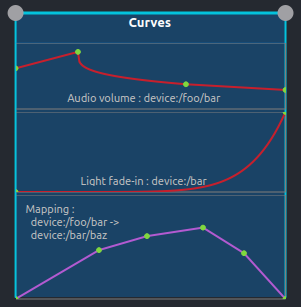
\includegraphics[scale=0.7]{images/curves.png}
        	\caption{Various kinds of curves}
        \end{figure}    
        
    \end{frame}
    
    \begin{lrbox}{\codebox}
    	\begin{lstlisting}
function(t) { 
    var obj = new Object; 
    obj["address"] = 'dev:/foo/bar'; 
    obj["value"] = t + iscore.value('other:/baz'); 
    return [ obj ]; 
}
    	\end{lstlisting}
    \end{lrbox}
    
    \begin{frame}
    	\frametitle{JavaScript}
    	\begin{figure}
    		\centering
    	    \usebox{\codebox}
    	    \caption{Called at each tick}
    	\end{figure}
    	
    	\begin{itemize}
    		\item Uses Qt's QJSEngine.
    		\item For now API with a single function : should be extended.
    	\end{itemize}
    \end{frame}
    
    \begin{frame}
        \frametitle{Hierarchy}
        
        \begin{figure}
        	\centering
        	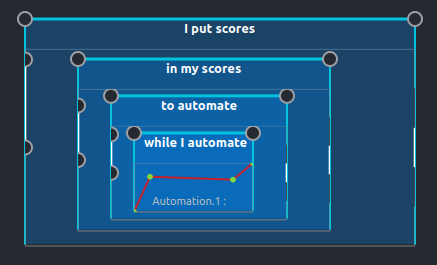
\includegraphics[scale=0.6]{images/hierarchy.png}
        	\caption{Scenarios can be nested arbitrarily}
        \end{figure}   
    \end{frame}
    
    \begin{frame}
        \frametitle{WIP : Spatial automations}
        
        \begin{figure}
        	\centering
        	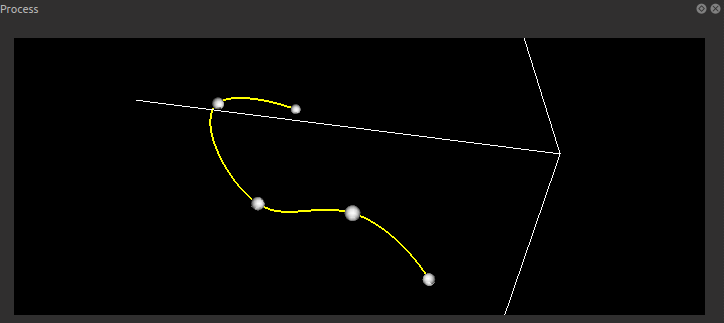
\includegraphics[width=\textwidth]{images/autom3d.png}
        \end{figure}   
        
        \begin{itemize}
        	\item 3d splines that uses VTK. Can be used to create paths in space for instance.
        	\item Spatial mappings to compute collisions, distances, etc. and performs actions according to the result of such computations.
        \end{itemize}
    \end{frame}
    

\begin{frame}
    \frametitle{Future : distribution ?}
    
    \Large
    \begin{itemize}
    	\item Currently : multiple instances can work together at the editing stage.
    	\item Soon : distributed execution.
    	\item Example scenarios :
    	\begin{itemize}
    		\item \large  100 phones controlling a parameter together.
    		\item Live backups if a computer dies during performance.
    		\item Offloading.
    	\end{itemize}
    	 
    \end{itemize}
\end{frame}

\begin{frame}
    \frametitle{Future : other features}
    \Large
    \begin{itemize}
    \item MIDI, WebSockets support
    \item Some level of patching, like Pd
    \item Complete remote-control abilities.\\ Currently : execution can be followed via a web page.
    \item Port excecution engine to FPGA. 
    \item Audio engine ? 
    \end{itemize}
\end{frame}

\begin{frame}
    \frametitle{Contributing}   
    \large 
    \begin{itemize}
    \item UX, UI (mock-ups were done but not entirely implemented)
    \item Documentation, writing demo scenarios
    \item Translations    
    \item Implement the Minuit protocol in your software with the OSSIA API    
    \item Many "low-hanging fruit" TODOs
    \item Mobile devices ports : 
    \begin{itemize}
        \item Android : builds and run but requires adapted UI.
        \item Web port : with PNaCl, runs but crashes. Will open the way to WebAssembly. 
        \item iDevices (many artists use them).
    \end{itemize}
\end{itemize}
    
\end{frame}



\begin{frame}
    \frametitle{Links}
    \begin{itemize}
        \item \textbf{Grab a release !} ~\\ \url{github.com/OSSIA/i-score/releases}. 
        \item \textbf{Protocols and implementations} :~\\
        \url{github.com/OSSIA}
    \end{itemize}
        
    \centering
    \vspace{2cm}
    \Large{Thanks ! Questions ?}
    \vspace{2cm}
    
    \small{Credits: 'simple' Beamer theme, Facundo Muñoz; Fira font}
\end{frame}    
\end{document}
